\documentclass{article}
\usepackage[left=2cm,right=2cm,top=3cm,bottom=3cm]{geometry}
\usepackage[polish]{babel}
%\usepackage[cp1250]{inputenc}
\usepackage{polski}
\usepackage{fancyhdr}
%\usepackage{amssymb}
%\usepackage[T1]{fontenc}
%\usepackage{lingmacros}
%\usepackage{tree-dvips}
\usepackage{graphicx}
\graphicspath{ {./img/} }
\usepackage{wrapfig}
\usepackage{array}
\usepackage{makecell}
\usepackage{subcaption}
\usepackage{hyperref}


%\renewcommand{\cellalign/theadalign}{vh}

\frenchspacing
\begin{document}
\pagestyle{fancy}
\fancyhead[LE,RO]{Mariusz Sendyk, Jakub Solich}
\fancyhead[LO,RE]{Mechatronika}
    \section{Cel projektu}
    Celem projektu jest zbudowanie klawiatury komputerowej w układzie
    ANSI TKL. Za pracę klawiatury odpowiadać będzie mikrokontroler, który zajmie się 
    komunikacją z komputerem poprzez USB.
    Głównym wyzwaniem projektu jest stworzenie kompletnego układu mikrokontrolera oraz programu
    w postaci modułu, do którego można będzie przyłączyć matrycę przycisków.

    \section{Założenia projektu}
    Na podstawowe założenia projektu składają się:
        \begin{itemize}
            \item Układ klawiatury w układzie ANSI TKL
            \item Komunikacja z komputerem poprzez USB
            \item Pooling rate 500Hz lub więcej
            \item Programowy de-bouncing
            \item Wspomaganie adresowania matrycy przełączników przy pomocy układów 74AHC138
            \item Wsparcie NKRO
        \end{itemize}
    Na dodatkowe założenia projektowe składają się:
        \begin{itemize}
            \item Obsługa makr
            \item Sterowanie podświetleniem poprzez moduł
            \item Mini system operacyjny
        \end{itemize}
    \section{Wybór rozwiązania projektowego}
    Praca klawiatury komputerowej w głównej mierze sprowadza się do ciągłego wykonywania następujących
    czynności przez mikrokontroler:
    \begin{enumerate}
        \item Pobierz stany przełączników (np. wykrycie stanu wysoki/niski na pinach)
        \item Na podstawie danych, wygeneruj kolejkę zmian przycisków (downstroke i upstroke, scancode)
        \item Prześlij dane do komputera/hosta
    \end{enumerate}
    Oczywiście to jest najsurowsza pętla pracy klawiatury. Jako układy wykonawczy postanowiono wykorzystać
    układ ATMega32U4. Jest to mikrokontroler firmy Atmel (obecnie pod Microchip), który jest szeroko stosowany
    w układach hobbystycznych. Układ ma ten następujące cechy, decydujące o jego zastosowanu:
    \begin{itemize}
        \item Duża wydajność obliczeniowa (głównie istrukcje wykonywane w 1 cyklu zegara oraz maks 16MHz)
        \item Sprzętowe USB dające sporo możliwości
        \item Bogate wyposażenie tj. 4 liczniki,  I\textsuperscript{2}C, SPI, tryby uśpienia, 2 pełne 8-bitowe porty I/O
        \item Zintegrowany stabilizator 3,3V, wymagany dla komunikacji z USB
        \item Bogata dokumentacja i obecność gotowych rozwiązań OpenSource (GH60) opatych na tym układzie
        \item Przyjazna w lutowaniu obudowa TQFP44
        \item I przede wszystkim spora ilość projektów klawiatur OpenSource opartych na tym układzie
    \end{itemize}
    Wybrany mikrokontroler posiada 44 piny. Standardowy układ ANSI posiada 104 klawisze. Z góry widać, że bezpośrednie
    podłączenie przycisków do pinów mikrokontrolera nie wystarczy. Zamiast takiego podejścia stosuje się \emph{matrycę przełączników}.
    \newpage
    \begin{figure}[h]
        \centering
        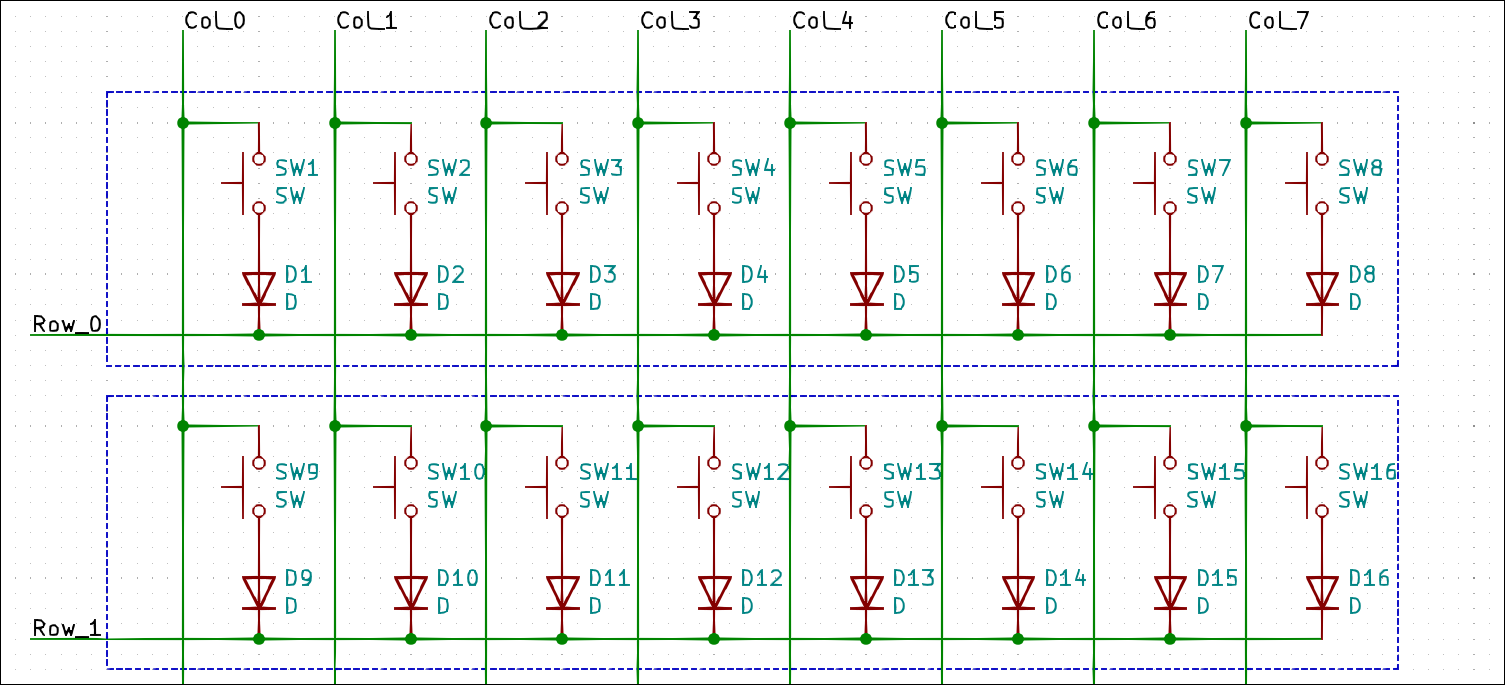
\includegraphics[width=0.6\textwidth]{1}
        \caption{Przykład matrycy przełączników}
    \end{figure}
    Połączenie przełączników w matrycę pozwala na adresowanie wybranej kolumny przycisków, a następnie ich odczytu.
    Ponieważ podczas odczytu musi być aktywna tylko jedna kolumna, to atrakcyjnym jest zastosowanie dekoderów n do n\textsuperscript{2}.
    Przykładowymi układami mogą być 74HC154 lub 74AHC138. Pierwszy układ to dekoder 4-do-16, zamienia 4 bitową wartość
    na wejściach na 1 z 16 na wyjściach. Aktywne wyjście przyjmuje stan niski, co pozwala na zastosowanie go bezpośrednio w układzie.
    Układ 74AHC138 jest tym samym układem co 154, ale 3-do-8. Oba układy posiadają możliwość łączenia w celu rozszerzenia
    ilości linii. Układ 154 byłby idealny, ponieważ 8*16 daje 128 klawiszy. Niestety, układ ten jest już stary 
    i dostępny jedynie w starym procesie technologicznym HC(T), który posiada duże opóźnienia (mogą one przekroczyć 
    50ns) i pobiera więcej energii (chociaż i tak pobierana energia jest znikoma). 74AHC138 natomiast, jest dostępny
    w procesie AHC, który jest znacznie szybszy (wszelkie opóźnienia nie przekraczają 10ns) i łatwiej dostępny.
    Układ ten również można rozszerzyć do 5-do-32. W naszym przypadku jedynie potrzebne jest 16 linii, ale nic nie
    stoi na przeszkodzie, by układ rozubodwać.
    \begin{figure}[h]
        \centering
        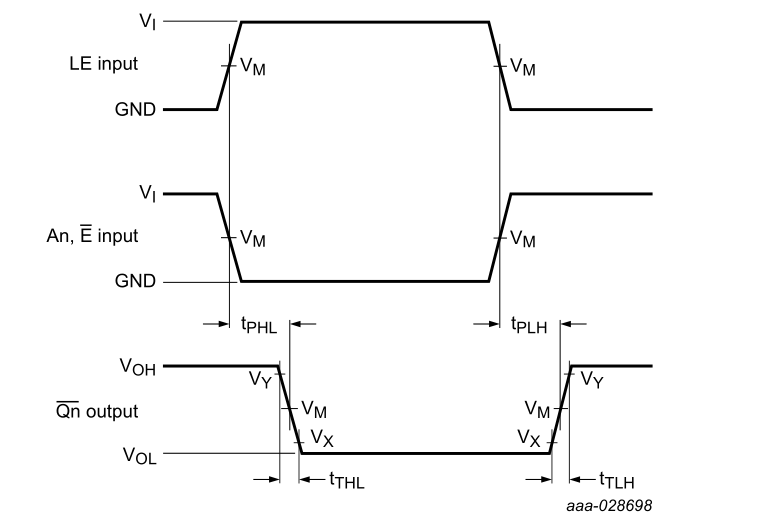
\includegraphics[width=0.4\textwidth]{2}
        \caption{Diagram czasowy}
    \end{figure}
    \begin{center}
        \begin{tabular}{ |c|c|c|c|c| }
            \hline
            \thead{Oznaczenie} & \thead{Opis} & \thead{Tpd} & \thead{Tt} & \thead{Warunki\\An do Qn}  \\ 
            \hline
            74HC4515 & \makecell{4-to-16 line decoder/demultiplexer with input latches;inverting} & 50ns & 15ns  & \makecell{4,5V}  \\
            \hline
            74HC154 & \makecell{4-to-16 line decoder/demultiplexer} & 30ns & 15ns  & \makecell{4,5V}  \\ 
            \hline
            74AHC138 & \makecell{3-to-8 line decoder/demultiplexer; inverting} & 10.1ns & N/A  & \makecell{4,5-5,5V} \\
            \hline
        \end{tabular}
    \end{center}

    \begin{center}
        \begin{tabular}{ |c|c|c|c|c|c|c|c|c| }
            \hline
            \thead{Producent} & \thead{SKU} & \thead{n-pin} & \thead{Flash} & \thead{SRAM} & \thead{EEPROM} & \thead{Wydajność} & \thead{Napięcie} & \thead{Peryferia}\\ 
            \hline
            Atmel/Microchip & ATMega32U4 & 44 & 32KB & 2,5KB & 1KB & 16MIPS & 2,7-5,5V & \makecell{USB\\JTAG\\SPI\\TWI\\USART\\ADC}\\
            \hline
            NXP & MC9S08JM60 & do 64 & do 60KB & do 4KB & N/A & 48MHz &  2,7-5,5V & \makecell{USB\\SPI\\TWI\\ADC\\RTC}\\ 
            \hline
            Microchip & PIC18F47J13 & 44 & 128KB & 3760B & N/A & 12MIPS & 2-3,6V & \makecell{USB\\SPI\\TWI\\RTCC\\ADC}\\
            \hline
        \end{tabular}
    \end{center}
    Co do mikrokontrolera to są jeszcze inne opcje. Poza mikrokontrolerami AVR8 firmy Atmel całkiem niemałą popularnością cieszą się
    układy innych firm, takie jak uC z serii PIC firmy Microchip oraz nieco bardziej skomplikowane (ale wydajniejsze) STM32 firmy ST.
    Z jakich powodów wybrany został uC ATMega32U4 to już zostało przedstawione.
    \section{Schemat blokowy}
    \begin{figure}[h]
        \centering
        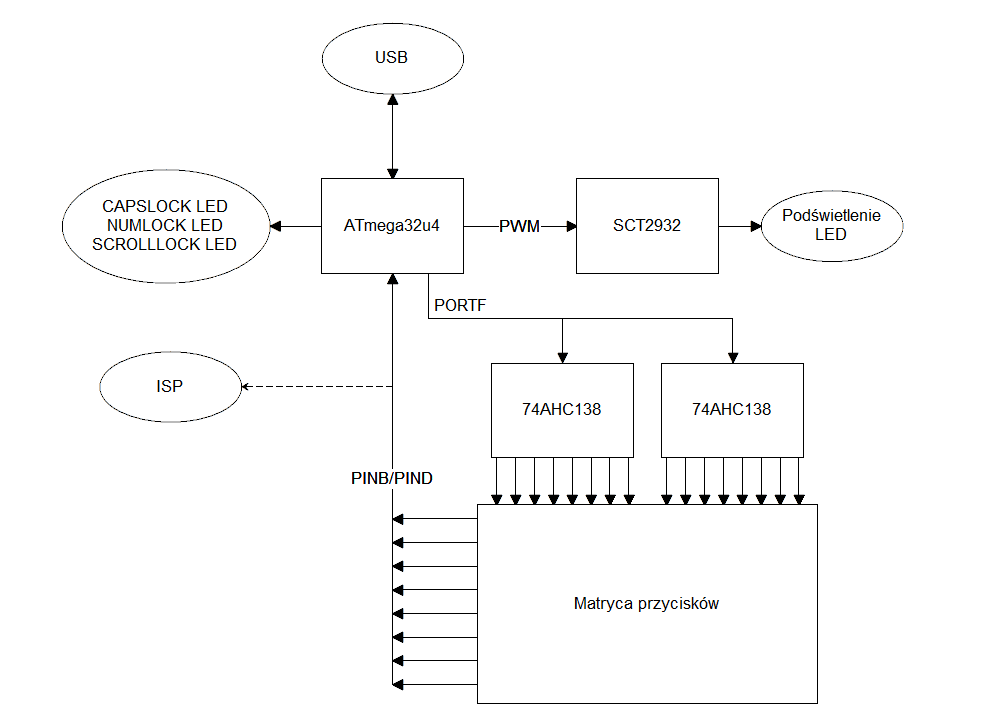
\includegraphics[width=0.8\textwidth]{3}
    \end{figure}
    \newpage
    Schemat blokowy układu wygląda następująco:
    \begin{itemize}
        \item Sercem płytki jest mikrokontroler ATMega32U4
        \item 4 piny z portu F są wykorzystywane do adresowania matrycy przycisków
        \item Odczyt z macierzy odbywa się poprzez wykorzystanie jednego lub dwóch pełnych portów B/B+D
        \item Pin C6 jest wykorzystywany jako wyjście dla sygnału PWM i jest on podłączony bezpośrednio do driver'a podświetlenia
        \item Jeśli do odczytu macierzy wykorzystuje się tylko jeden port (B), to wówczas linie portu D mogą być wykorzystane do innych celów
        \item 3 piny uC są dedykowane do obsługi kontrolek Caps Lock, Num Lock, Scroll Lock
    \end{itemize}
    Powyższy schemat blokowy zrealizowano w postaci schematu:
    \begin{figure}[h]
        \centering
        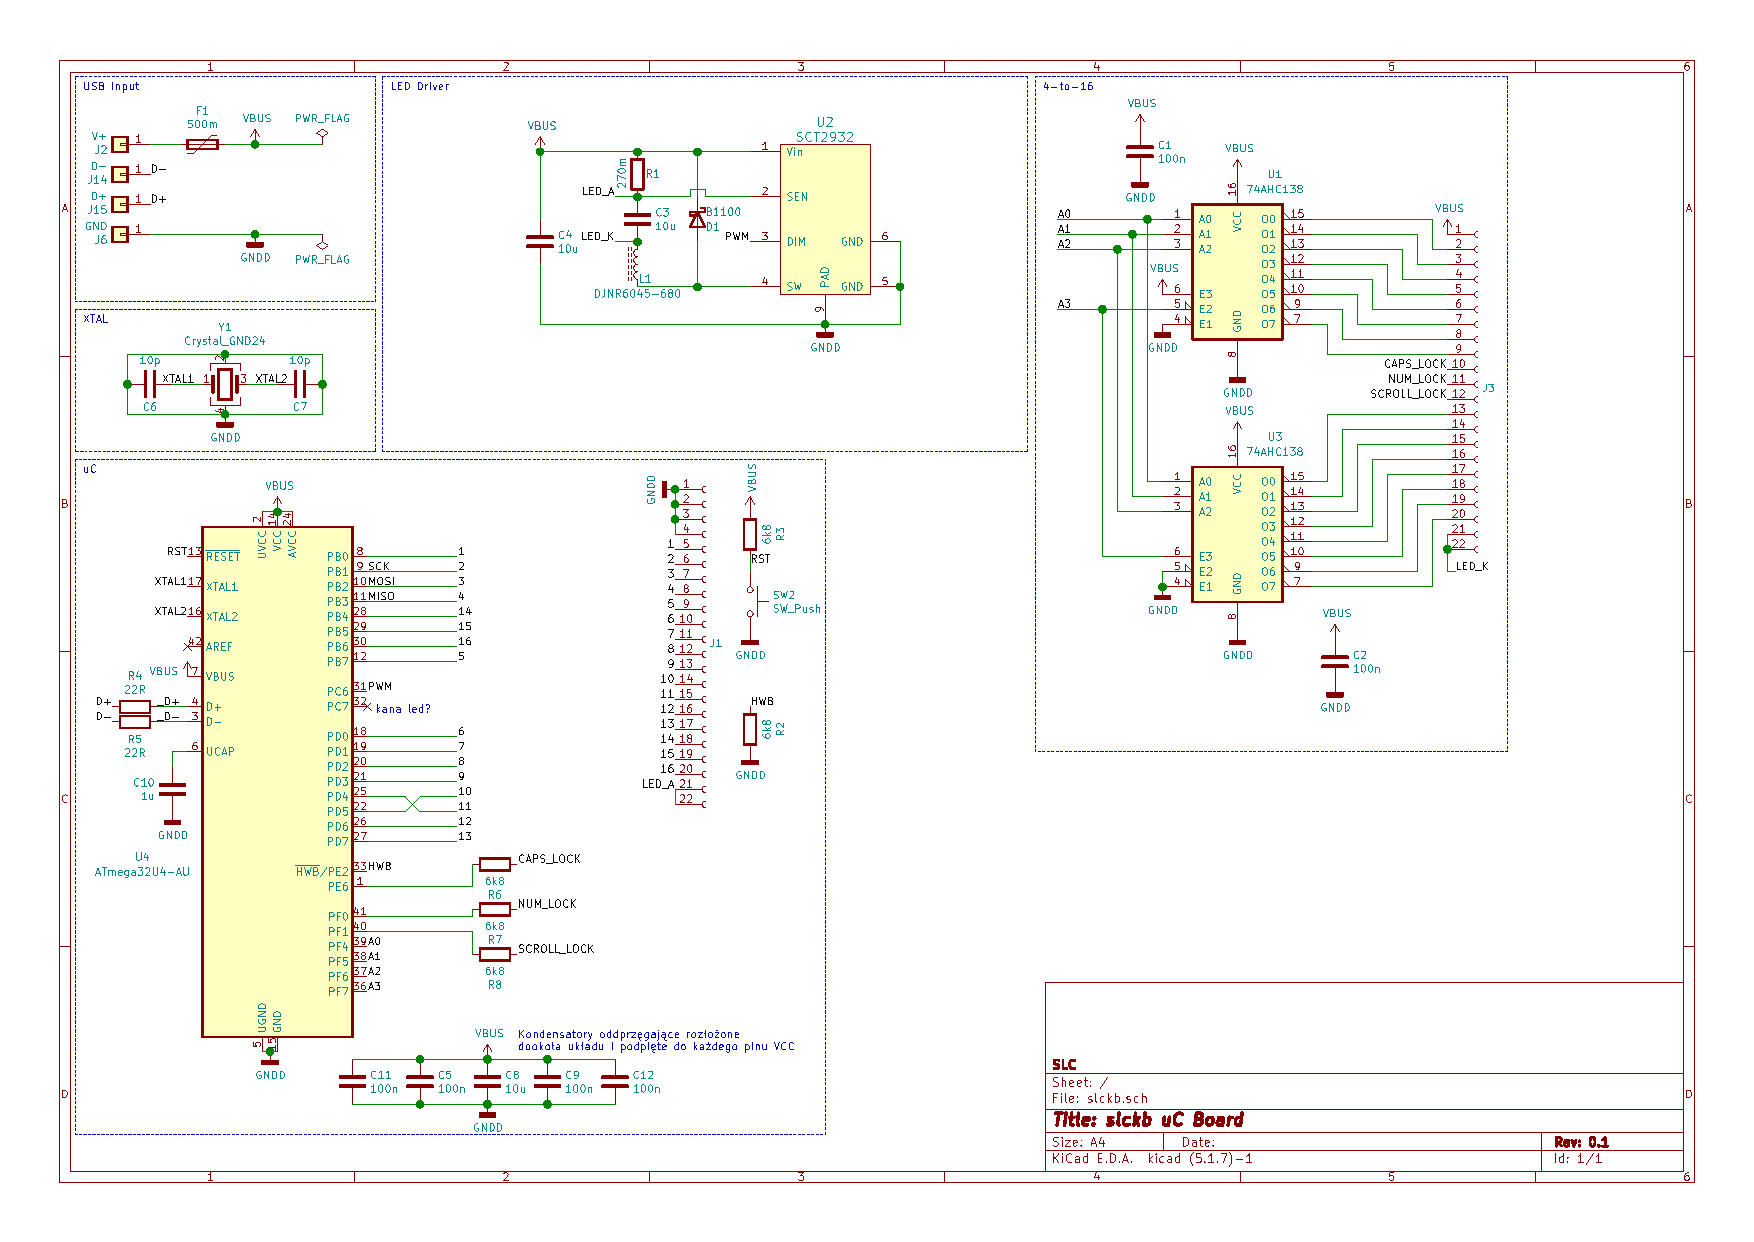
\includegraphics[width=\textwidth]{slckb.pdf}
    \end{figure}
    \newpage
    A następnie płytki drukowanej:
    \begin{figure}[h]
        \centering
        \begin{subfigure}{0.3\textwidth}
            \centering
            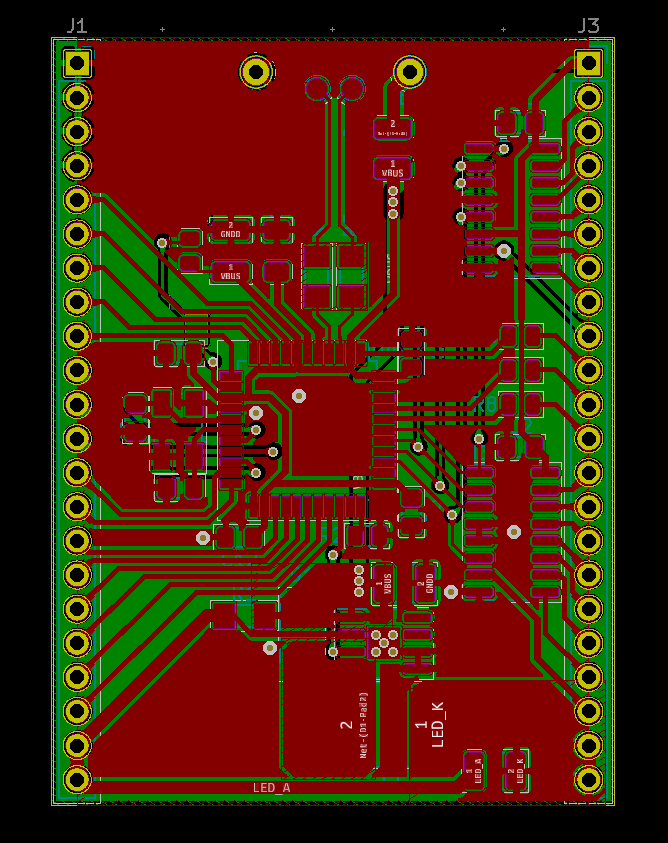
\includegraphics[height=6cm]{pcb.png} 
            \caption{Rysunek płytki}
            \label{fig:subim1}
            \end{subfigure}
        \begin{subfigure}{0.3\textwidth}
            \centering
            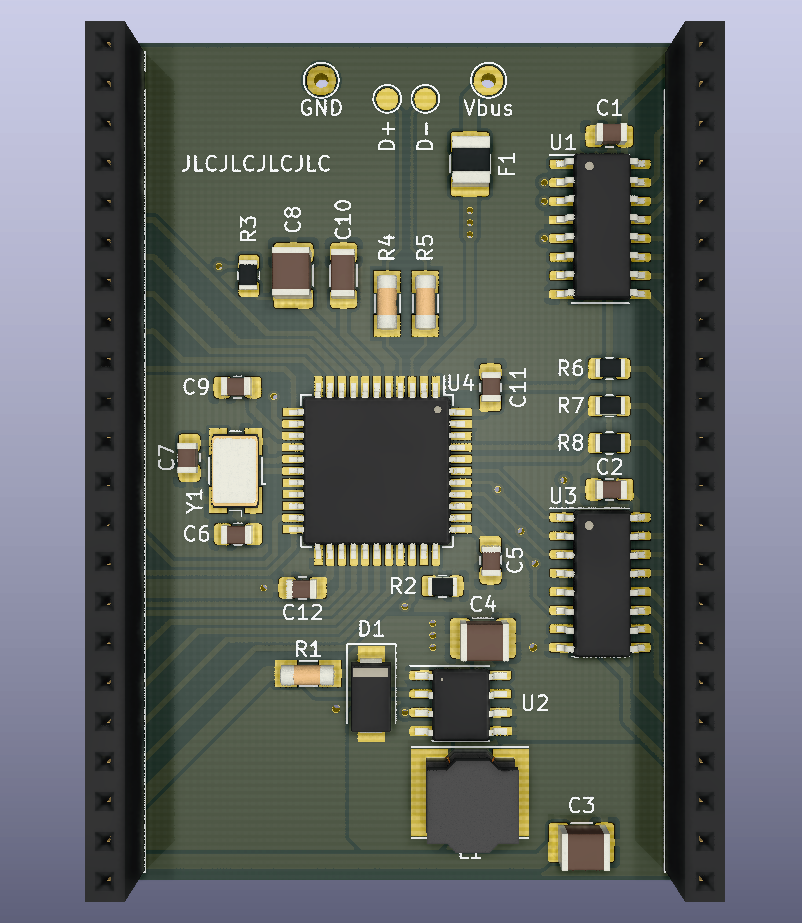
\includegraphics[height=6cm]{pcb2}
            \caption{Render płytki góra}
            \label{fig:subim2}
        \end{subfigure}
        \begin{subfigure}{0.3\textwidth}
            \centering
            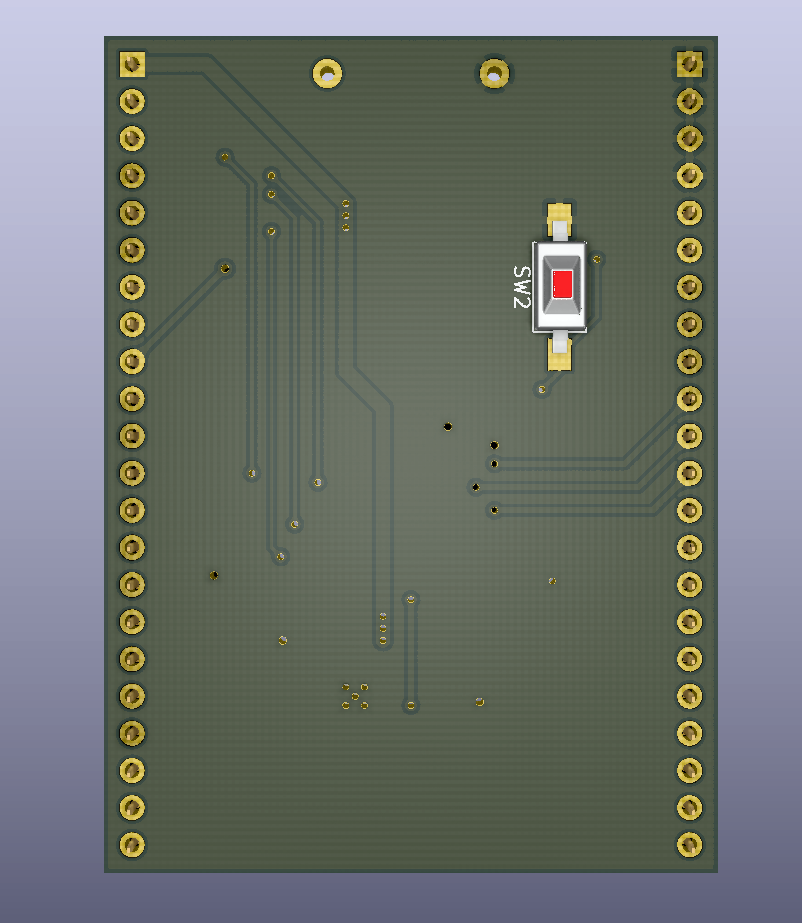
\includegraphics[height=6cm]{pcb3}
            \caption{Render płytki dół}
            \label{fig:subim3}
        \end{subfigure}
        \end{figure}

    Tak jak widać, można zauważyć przycisk na spodzie płytki. Cała płytka ma pełnić rolę modułu, który jest wpinany w płytkę PCB
    z przełącznikami. Sam rozstaw listw pinów nie jest przypadkowy, ponieważ wynosi on 1,5 cala, co jest równe 2u (u - unit - jednostka).
    Jeden u w terminologi klawiatur jest równe 0,75", i taka odległość dzieli centra przełączników. Innymi słowy moduł ten powinien 
    zmieścić się pomiędzy rzędy przełączników. Z tego właśnie powodu jest przycisk na spodzie płytki, aby łatwo możnabyło zresetować
    układ mikrokontrolera i przejść w tryb DFU (tryb w którym można programować układ bezpośrednio z USB). Dodatkowo na płytce znajduje się
    jeszcze bezpiecznik polimerowy 500mA.
    \section{Układ podświetlenia}
    Poza układami 74AHC138 na płytce znajduje się jeszcze układ SCT2932 firmy Starchip. Jest to jeden z wielu układów przeznaczonych do zasilania
    LED stałym prądem. Układ ten został wybrany z kilku następujących powodów:
    \begin{itemize}
        \item Może pracować od 5 do 33V
        \item Bardzo prosta konstrukcja
        \item Możliwość sterowania jasnością poprzez PWM
        \item Zabezpieczenie termiczne, przeciwzwarciowe i soft-start
        \item Wymaga tylko 4 komponentów zewnętrznych
        \item Możliwość pracy do 1,5A prądu wyjściowego
        \item Prąd jest ustalany poprzez dobranie rezystora
        \item 0.1V napięcia odniesienia - niski dropout
    \end{itemize}
    Układ domyślnie miał pracować z rezystorem 270mOhm co powinno dać 370mA prądu. Przy tej wartości został zbadany układ w celu
    ocenienia jego sprawności. Ostatecznie zaobserwowano:
    \begin{itemize}
        \item Sprawność bardzo mocno zależy od odsprzęgnięcia zasilania układu (C4), dlatego wykorzystano kondensator SMD MMLC 1210 X7R 10uF
        \item Sprawność zależy od różnicy między napięciem wejściowym zasilania a wyjściowym (im mniejsza różnica tym wyższa sprawnośc)
        \item Białe diody LED przy prądzie 370mA potrzebowały 2,75V (przy niższym prądzie wartość ta będzie niższa oczywiście)
        \item Najwyższa zmieżona sprawność to ~75\%, jednakże należy mieć na uwadze, że oba kondensatory (C4 i C3) nie były dobrze połączone z układem
    \end{itemize}
    Teoretyczna sprawność powinna spokojnie zaczynać się od 80\% dla wyższych prądów (powyżej 150mA). Wartości komponentów zewnętrznych są takie same jak
    te opisane w nocie katalogowej układu. Przy powyższych warunkach zmierzono również częstotliwość z jaką pracuje układ (zależy ona głównie od stosunku Vin do Vout)
    i wyniosła ona około 100kHz.
    \begin{figure}[h]
        \centering
        \includegraphics[width=\textwidth]{scope.png}
        \caption{Napięcie na wyjściu tranzystora kluczującego. Stan niski oznacza przewodzenie}
    \end{figure}
    \section{Program}
    Napisanie programu dla klawiatury jest jednocześnie łatwym i trudnym zadaniem. Wszystko zależy od interfejsu klawiatura-komputer.
    Starsze klawiatury (i myszki) posługiwały się portem PS/2 (jeszcze starsze AT), który pomimo swoich zalet, został już prawie całkowicie wyparty.
    Główną zaletą PS/2 była prostota przesyłu danych po dwóch liniach. Warstwa fizyczna nie wymaga dedykowanego układu, a protokół jest relatywnie prosty
    do implementacji w programie.\newline
    Jeśli chodzi o USB to sprawa jest odwrotna. USB jest stworzone by być uniwersalne i przez to nawet najprostsza rzecz jak klawiatura i mysz
    wymagają pełnej implementacji protokołu, punktów końcowych, deskryptorów, ramek i pakietów. Z tego powodu postanowiono skorzystać z rozwiniętego
    projektu oprogramowania do klawiatur opartych na układach AVR i SMT32: QMK. QMK to bardzo kompleksowe rozwiązanie do zaprogramowania układu klawiatury.
    Główną siłą QMK jest jego elastyczność.
    Każda implementacja układu mikrokontrolera jest rozróżniania w folderze \path{firmware/qmk_firmware/keyboards}.
    W tym folderze znajdują się pliki, które modyfikują domyślny program tak, aby pasował on do naszego rozwiązania. W naszym przypadku jest to 
    \path{firmware/qmk_firmware/keyboards/slckb}.
    W domyślnej postaci urzytkownik musi jedynie określić piny wykorzystywane do skanowania matrycy (plik config.h), komponenty, które mają zostać skompilowane i
    dołączone do programu (rules.mk), keymapa (tłumacząca fizyczne położenie przycisku w matrycy na nasze) i układ/przypisanie przycisków.\newline
    Aby zmodyfikować QMK do potrzeb projektu, trzeba zdefiniować własną wersję funkcji wykonujących dane czynności tj. inicjacja matrycy i jej skan.
    W tym celu wykorzystano dokumentację dostępną na stronie projektu: \url{https://qmk.fm/} 
    Kod jest dobrze skomentowany i tłumaczy kolejne czynności.
    W pliku config.h można zdefiniować takie rzeczy jak: wymuszenie NKRO (false), interwał skanowania (1ms), czas debouncingu (3ms).
    \section{Prototyp}
    Po stworzeniu programu przyszedł czas na prototyp. Przy użyciu OpenSCAD stowrzona została płytka testowa, która mieści 17 przełączników.
    Cała płytka ma kształt i układ numpada. Płytka ta została wydrukowana na drukarce 3D.
    \begin{figure}[h]
        \centering
        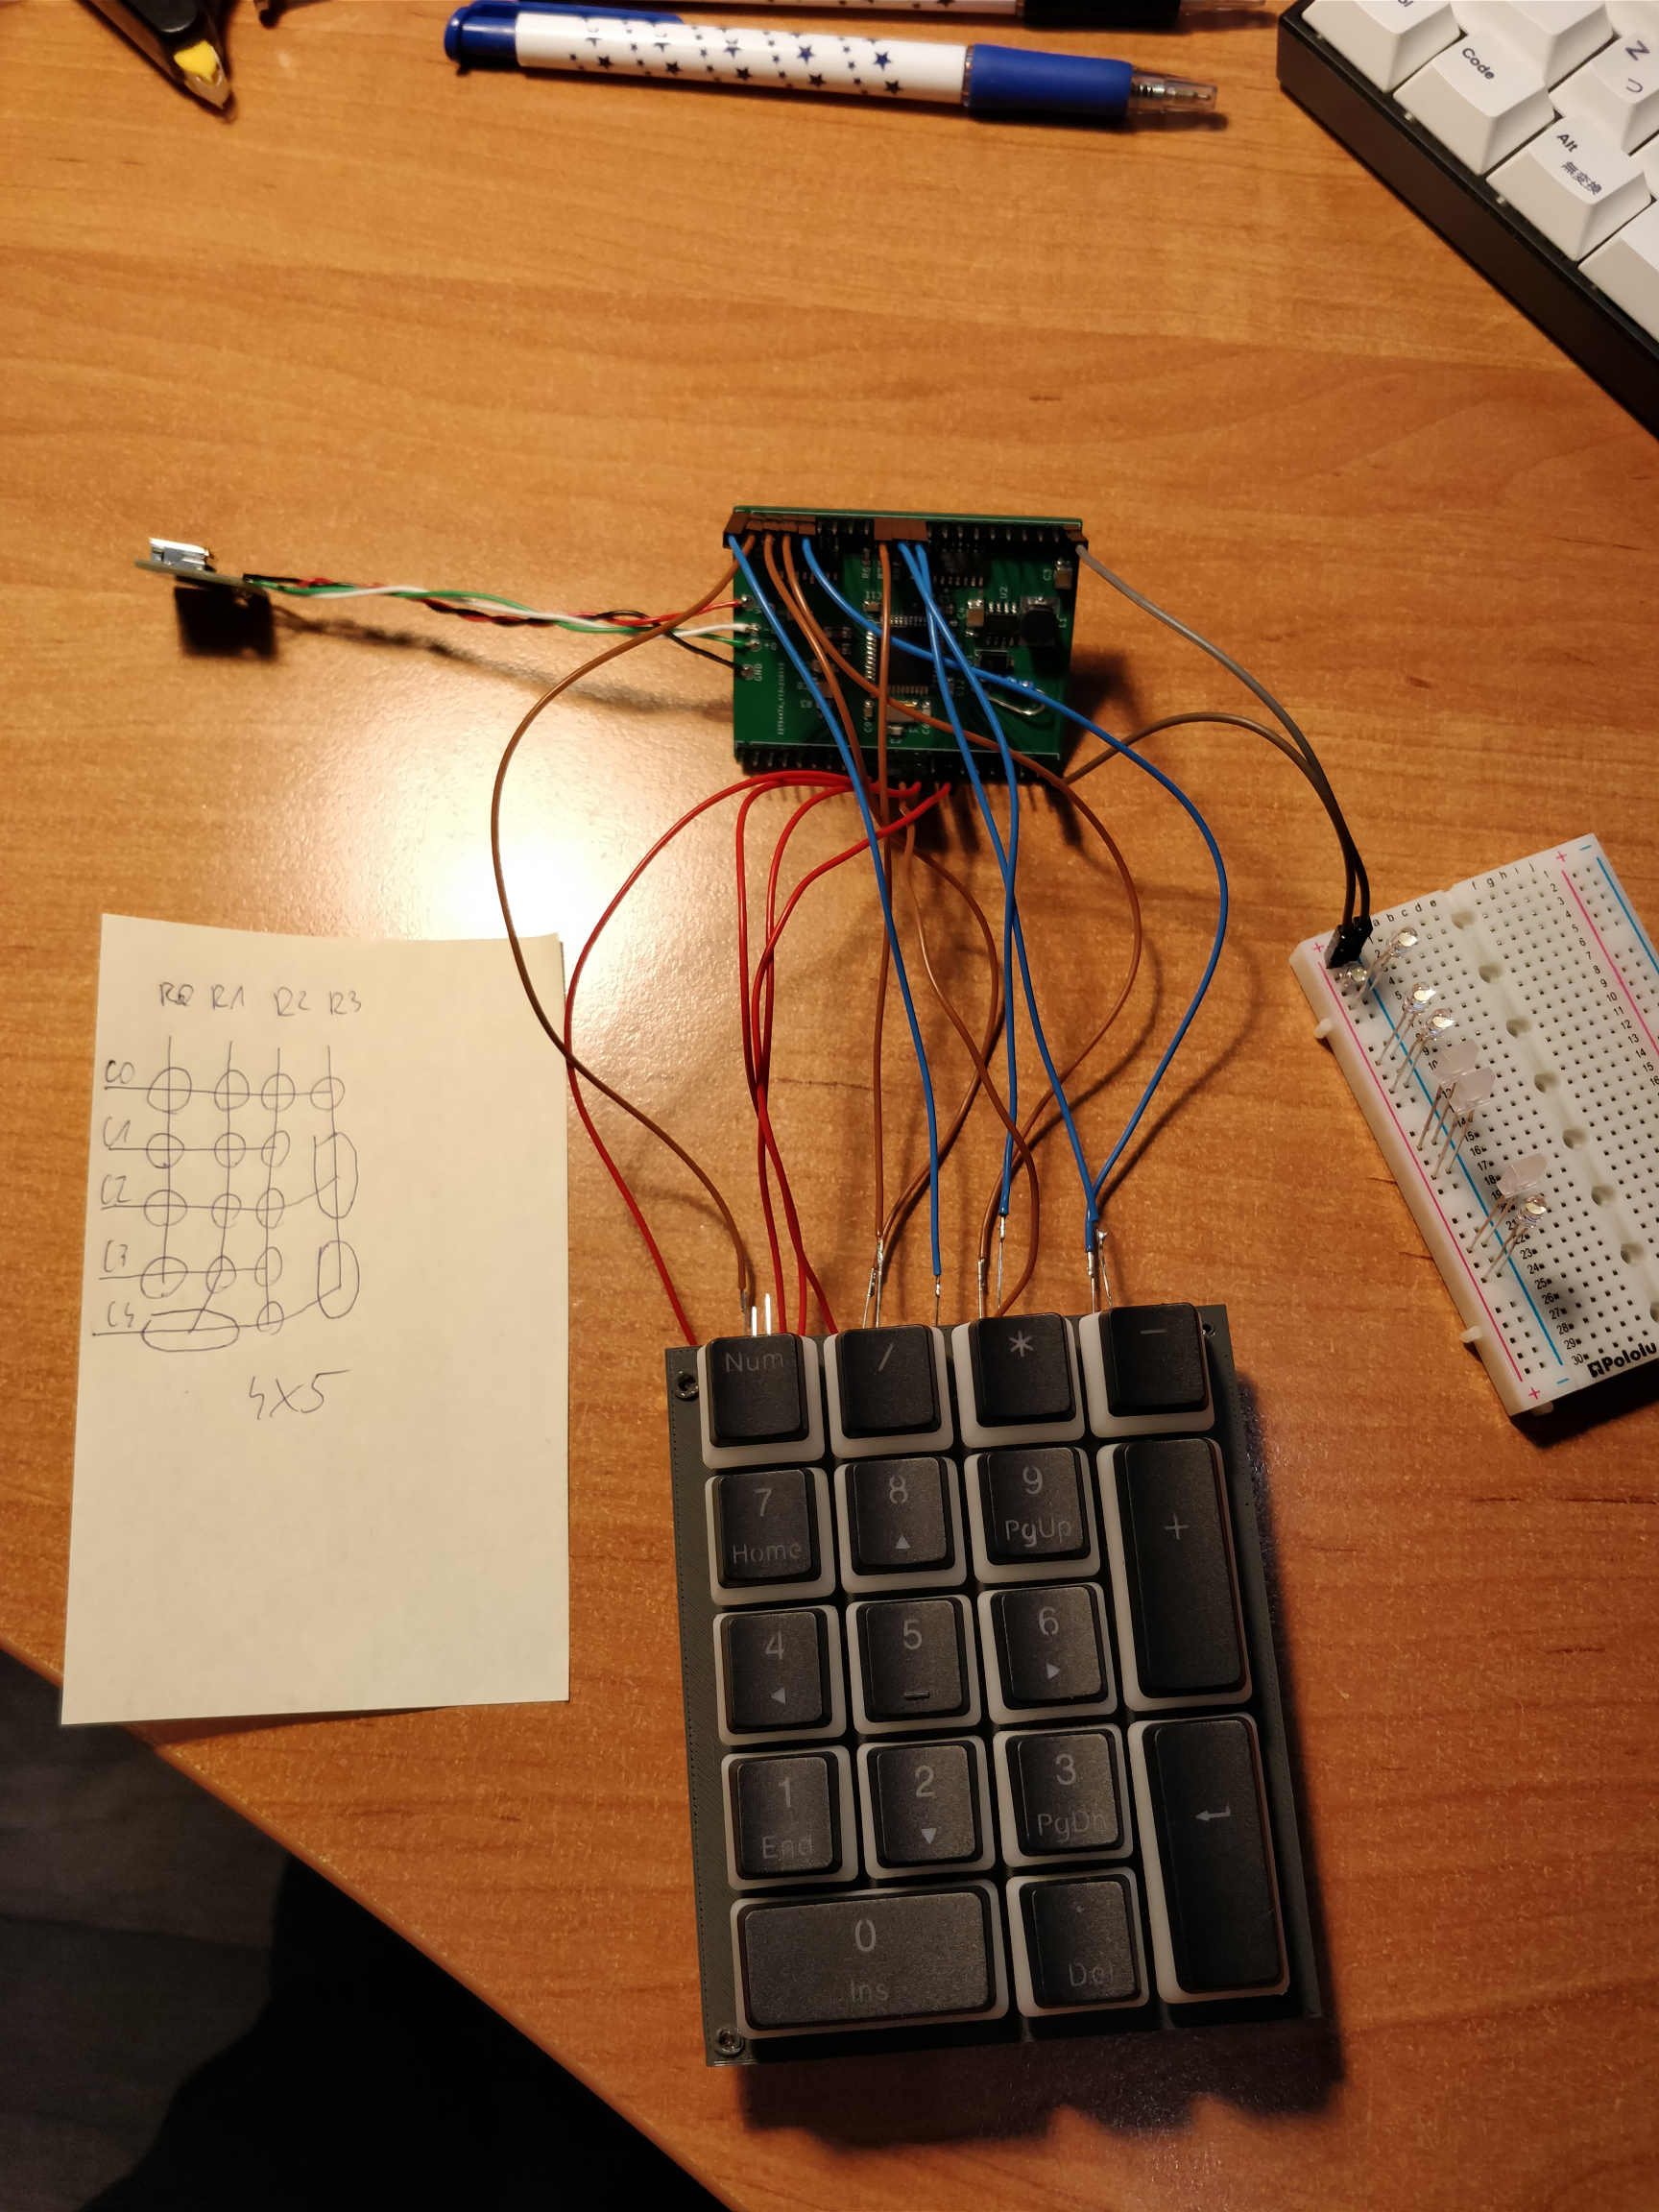
\includegraphics[width=0.5\textwidth]{proto.jpg} 
        \caption{Złożony prototyp wraz ze schematem połączenia}
        \end{figure}
    \newpage
    \begin{figure}[h]
        \centering
        \begin{subfigure}{0.45\textwidth}
            \centering
        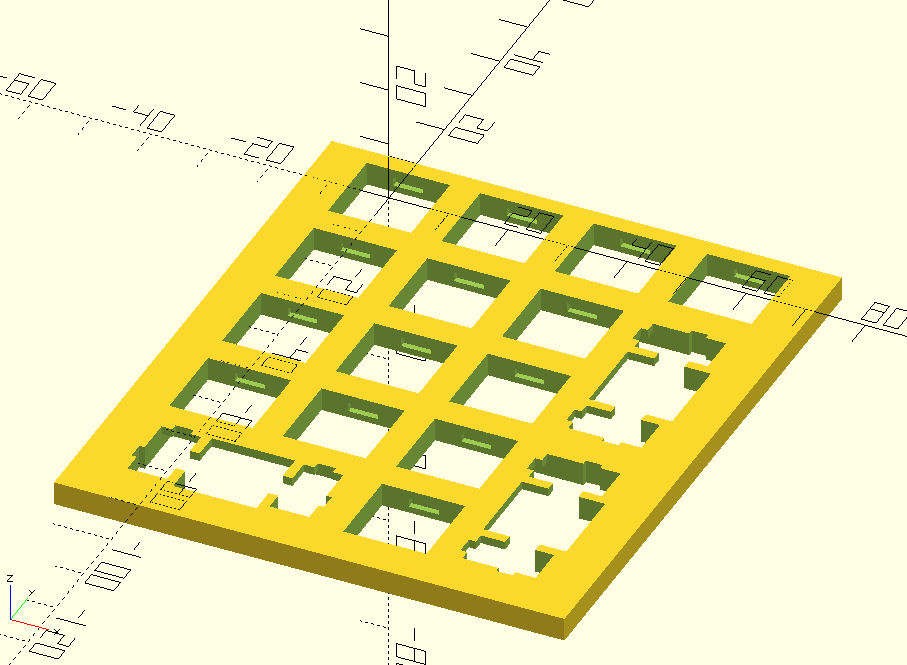
\includegraphics[height=5cm]{plate.png} 
        \caption{Model płytki montażowej}
        \label{fig:subim1}
        \end{subfigure}
        \begin{subfigure}{0.45\textwidth}
            \centering
            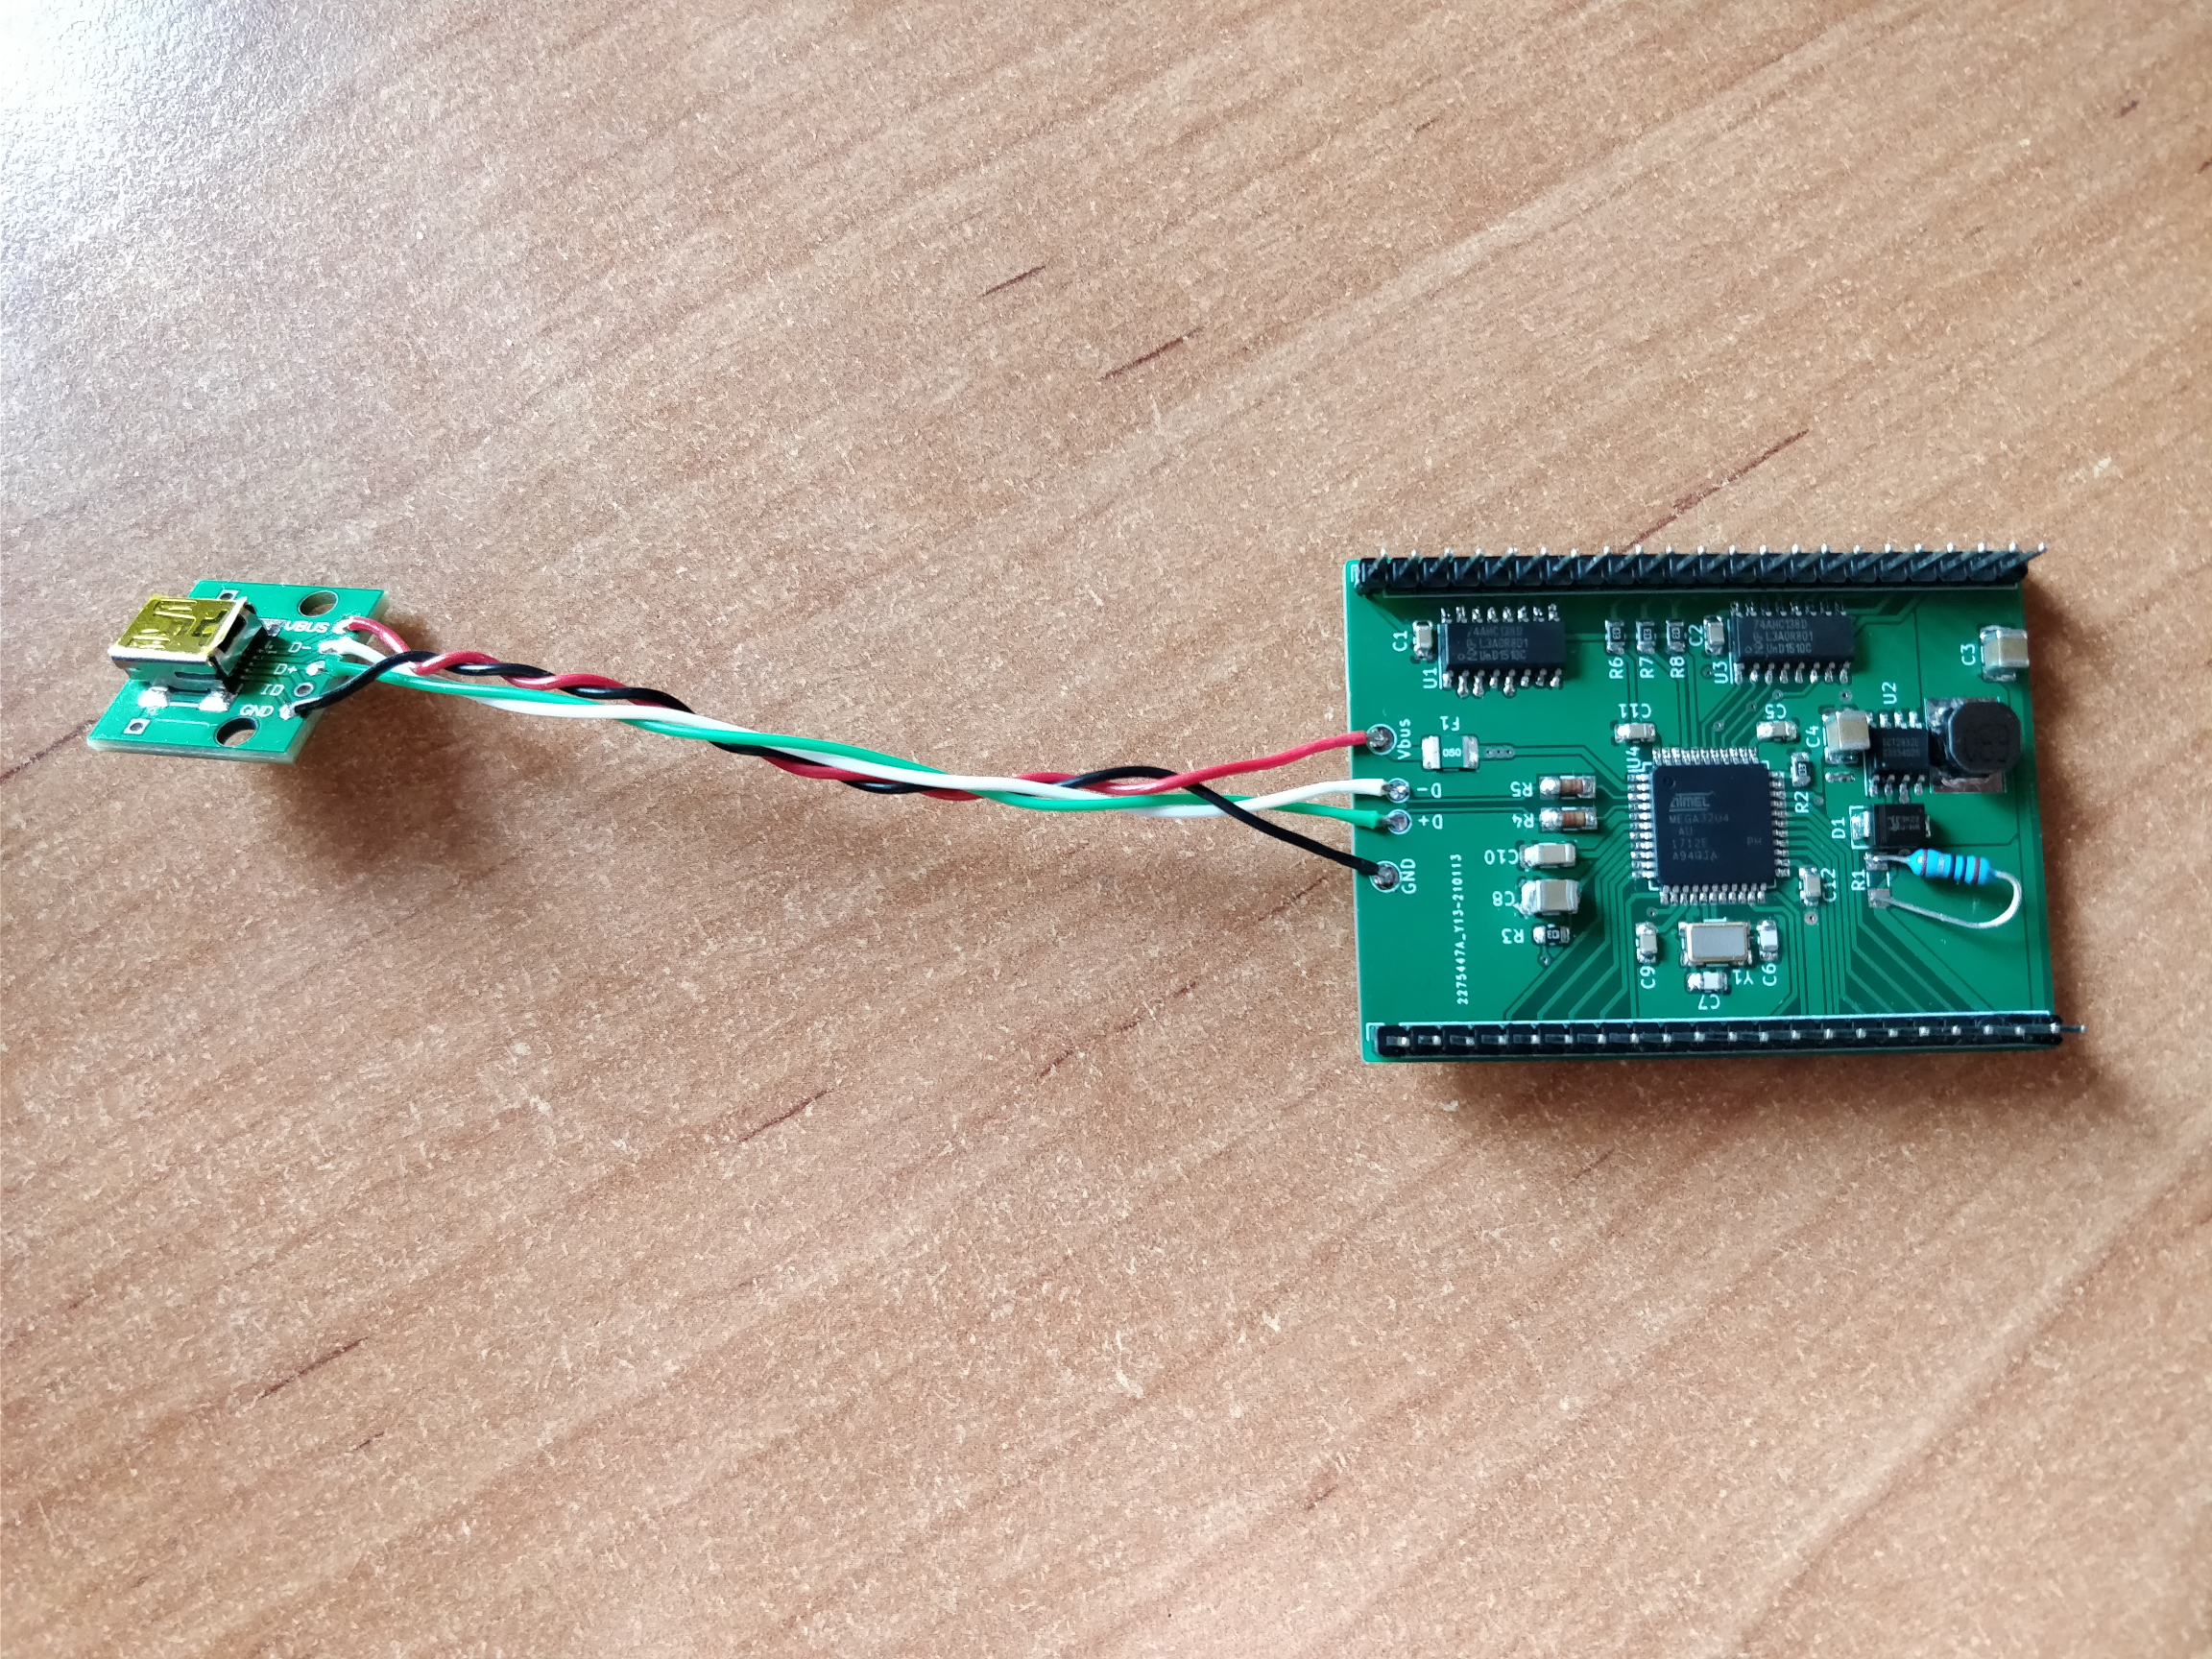
\includegraphics[height=5cm]{pcb_2.jpg}
            \caption{Złożone i zlutowane PCB}
            \label{fig:subim2}
        \end{subfigure}
        \end{figure}
    W prototypie zdefioniowano 2 wartstwy. Definicje warstw można znaleźć w pliku
    \path{firmware/qmk_firmware/keyboards/slckb/keymaps/default/keymap.c}

    \begin{figure}[h]
        \centering
        \begin{subfigure}{0.45\textwidth}
            \centering
        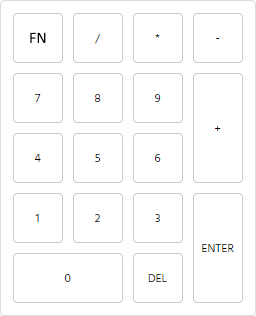
\includegraphics[height=5cm]{l1.png} 
        \caption{Warstwa główna}
        \label{fig:subim1}
        \end{subfigure}
        \begin{subfigure}{0.45\textwidth}
            \centering
            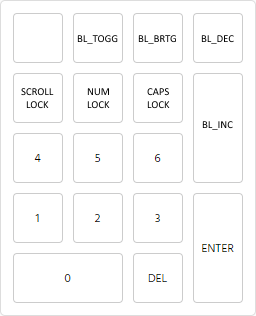
\includegraphics[height=5cm]{l2.png}
            \caption{Warstwa FN}
            \label{fig:subim2}
        \end{subfigure}
        \end{figure}
    Diody od kontrolek ScrollLock, CapsLock oraz NumLock zostały umieszczone pod przyciskami / , * , - .
    Ponieważ cały prototyp jest zlutowany metodą p2p, dodanie diód podświetlenia wprowadziłoby duży bałagan i możliwość zwarcia zasilania podświetlenia z
    obwodami matrycy. Z tego powodu za "podświetlenie" będzie służyć kilka diód połączonych równolegle w płytce stykowej.
    W ostateczności wszystko działa. Dzięki wykorzystaniu QMK zostały osiągnięte wszystkie założenia projektu za wyjątkiem układu klawiatury (numpad zamiast TKL).
    Jest to spowodowane delikatnym przerostem projektu oraz złego zarządzania czasem odnośnie prac nad poszczególnymi elementami projektu.
    Ostateczny produkt wraz z oprogramowaniem może zostać wykorzystane do budowy klawiatury o wymiarach matrycy 16x16, co daje 256 klawiszy. Oczywiście tak długo
    jak starczy pamięci programu oraz SRAM.
\end{document}
